% !TeX spellcheck = ru_RU_yo
%% -*- coding: utf-8 -*-
\documentclass[12pt,a4paper]{scrartcl} 
\usepackage[T1,T2A]{fontenc}
\usepackage[english,russian]{babel}
\usepackage[utf8]{inputenc}
\usepackage{geometry} 
\geometry{tmargin=2cm,bmargin=2cm,lmargin=3cm,rmargin=1.5cm}
\usepackage{indentfirst}
\usepackage{misccorr}
\usepackage{graphicx}
\usepackage{amsmath}
\usepackage{setspace}
\PassOptionsToPackage{hyphens}{url}
\usepackage[breaklinks]{hyperref}
\usepackage{minted}
\usepackage{textcomp}
\usepackage{comment}
\usepackage{soul}
\usepackage{array}
\usepackage{longtable}
\usepackage{multirow}
\usepackage{makecell}
\usepackage[stable]{footmisc}
\usepackage{tabularx,booktabs} 
\graphicspath{{images/}}
\usepackage{svg}
\svgpath{{images/}}

%Отключает нумерацию страницы
\pagestyle{empty}

%\titleformat*{\section}{\centering\bfseries}
%\titleformat*{\subsection}{\Large\bfseries}
%\titleformat*{\subsubsection}{\large\bfseries}
%\titleformat*{\paragraph}{\large\bfseries}
%\titleformat*{\subparagraph}{\large\bfseries}

% Команда для линии с нижним подчёркиванием, возможностью написания сверху текста на ней и текстом под ней.
\newcommand\superunderline[3]{$\underset{\text{#3}}{\text{\underline{\hspace{0.3cm}#1\hspace{#2}}}}$}

% Тоже самое, но ещё с отступом слева от текста (выравнивание по середине)
\newcommand\superunderlinec[3]{$\underset{\text{#3}}{\text{\underline{\hspace{#2}#1\hspace{#2}}}}$}

% "Прокаченные" типы колонок для LaTeX. Умеют выравнивать содержимое столбца по горизонтали и принимать фиксированный размер. Полезная вещь.
\newcolumntype{L}[1]{>{\raggedright\let\newline\\\arraybackslash\hspace{0pt}}m{#1}} % Выравнивание по левому краю.
\newcolumntype{C}[1]{>{\centering\let\newline\\\arraybackslash\hspace{0pt}}m{#1}} % Выравнивание по середине.
\newcolumntype{R}[1]{>{\raggedleft\let\newline\\\arraybackslash\hspace{0pt}}m{#1}} % Выравнивание по правому краю.

% Разработка 1993 года: команды, исправляющие неправильные отступы в шапке и подвале колонок в таблицах LaTeX. 
\newcommand\Tstrut{\rule{0pt}{2.6ex}}         % Введи \Tstrut если буквы в таблице налезли на верхнюю полоску
\newcommand\Bstrut{\rule[-0.9ex]{0pt}{0pt}}   % И \Bstrut если буквы "съехали" с середины колонки или наезжают на нижнюю полоску

%Настройки для того, чтобы была возможность переносить строки внутри таблиц. Подробнее здесь:  https://tex.stackexchange.com/questions/2441/how-to-add-a-forced-line-break-inside-a-table-cell
\renewcommand\theadalign{bc}
\renewcommand\theadfont{\normalfont}
\renewcommand\theadgape{\Gape[0pt]}
\renewcommand\cellgape{\Gape[0pt]}

% Убираем варнинг о том что long table представляет собой слишком большой vbox
\makeatletter
\def\LT@start{%
  \let\LT@start\endgraf
  \endgraf\penalty\z@\vskip\LTpre
  \dimen@\pagetotal
  \advance\dimen@ \ht\ifvoid\LT@firsthead\LT@head\else\LT@firsthead\fi
  \advance\dimen@ \dp\ifvoid\LT@firsthead\LT@head\else\LT@firsthead\fi
  \advance\dimen@ \ht\LT@foot
  \edef\restore@vbadness{\vbadness\the\vbadness\relax}% (added)
  \vbadness=\@M % (added)
  \dimen@ii\vfuzz
  \vfuzz\maxdimen
    \setbox\tw@\copy\z@
    \setbox\tw@\vsplit\tw@ to \ht\@arstrutbox
    \setbox\tw@\vbox{\unvbox\tw@}%
  \vfuzz\dimen@ii
  \restore@vbadness % (added)
  \advance\dimen@ \ht
        \ifdim\ht\@arstrutbox>\ht\tw@\@arstrutbox\else\tw@\fi
  \advance\dimen@\dp
        \ifdim\dp\@arstrutbox>\dp\tw@\@arstrutbox\else\tw@\fi
  \advance\dimen@ -\pagegoal
  \ifdim \dimen@>\z@\vfil\break\fi
      \global\@colroom\@colht
  \ifvoid\LT@foot\else
    \advance\vsize-\ht\LT@foot
    \global\advance\@colroom-\ht\LT@foot
    \dimen@\pagegoal\advance\dimen@-\ht\LT@foot\pagegoal\dimen@
    \maxdepth\z@
  \fi
  \ifvoid\LT@firsthead\copy\LT@head\else\box\LT@firsthead\fi\nobreak
  \output{\LT@output}%
}
\makeatother

%Используется для построения подчеркивающих линий
\newlength{\ML}

\setlength{\parskip}{0.5cm}

%\thispagestyle{empty}

\begin{document}
	\phantom{fake text for spacing}
	% ТИТУЛЬНАЯ ЧАСТЬ
	\begin{center}
		\textbf{Министерство науки и высшего образования Российской Федерации} \\
		\textbf{ФГАОУ ВО «Волгоградский государственный университет»} \\
		\textbf{Институт Математики и информационных технологий} \\
		\textbf{Кафедра компьютерных наук и экспериментальной математики} \\
		
		\vspace{0.6cm}
		
		\hfill\begin{minipage}{0.4\textwidth}
		\begin{flushright}
			\textbf{\textsc{УТВЕРЖДАЮ:}} \\
			Зав. кафедрой \textit{КНЭМ} \\
			Клячин В.А.\\
			«01» сентября 2021 г.
		\end{flushright}
		\end{minipage}
		
		\vspace{0.6cm}
		
		\textbf{
			ИНДИВИДУАЛЬНОЕ ЗАДАНИЕ на УЧЕБНУЮ ПРАКТИКУ, НАУЧНО-ИССЛЕДОВАТЕЛЬСКАЯ РАБОТА (ПОЛУЧЕНИЕ ПЕРВИЧНЫХ НАВЫКОВ НАУЧНО-ИССЛЕДОВАТЕЛЬСКОЙ РАБОТЫ)
			на 2021 - 2022 год
			\vspace{0.2cm}
		}
		
		\vspace{0.3cm}
		\renewcommand{\arraystretch}{1.5} %!!!
		
		\begin{tabular}{R{3cm}cc}
			Студент & \superunderlinec{\thead{Курбанов Эльдар \\ Ровшанович}}{1.0cm}{(ФИО)} &  \superunderlinec{\thead{МОСм-201}}{1.9cm}{(группа)}
			\vspace{0.6cm} \\
			Руководитель практики от ВолГУ & \superunderlinec{\thead{\phantom{fake text for align}\\Клячин В.А.}}{1.1cm}{(ФИО)} & \superunderlinec{\thead{зав. кафедрой КНЭМ,\\проф., д.ф.-м.н.}}{0.7cm}{(должность, ученое звание и степень)} \\
			Ответственный за организацию практики от кафедры
 & \superunderlinec{\thead{\phantom{fake text for align}\\Клячин В.А.}}{1.1cm}{(ФИО)} & \superunderlinec{\thead{зав. кафедрой КНЭМ,\\проф., д.ф.-м.н.}}{0.7cm}{(должность, ученое звание и степень)} \\
			%ragedleft?????? seriously, it works as right align. WTF????
			\multirow{3}{3cm}{\raggedleft Место прохождения практики} & \multicolumn{2}{c}{\underline{\hspace{0.2cm}Лаборатория <<Математического и программного обеспечения\hspace{1cm}}} \\
			& \multicolumn{2}{l}{\superunderlinec{\hspace{0.2cm}ЭВМ>> кафедры КНЭМ ИМИТ ФГАОУ ВолГУ\hspace{3.7cm}}{0cm}{(наименование учреждения, структурного подразделения)}} \\
			Сроки прохождения практики & \multicolumn{2}{c}{с <<01>> сентября 2021 г. по <<30>> декабря 2021 г.}
		\end{tabular}
	\end{center}
	%КОНЕЦ ТИТУЛЬНОЙ ЧАСТИ
	
	\vspace{0.2cm}
	%1 раздел
	1. Содержание и задания практики:
		%\newpage
		\begin{longtable}{| L{0.7cm} | L{1.9cm}| L{3.3cm} | L{1.2cm} | L{2.1cm} | L{3.5cm} |}
			\hline % Требуется для рисования горизонтальной линии.
			\centering{№ п/п} &	\centering{Этапы практики} & \centering{Содержание работы и задания этапов} & \Tstrut \centering{Коли-чество часов} & \Tstrut \centering{Календар-ные сроки проведе-ния} & Форма отчетности \\
			\hline
			% Используем Bstrut и Tstrut в необходимых местах чтобы чинить вёрстку таблицы. Как можете заметить, выше пришлось вручную переносить слова при помощи "-". К сожалению, Bstrut и Tstrut ломают автоматические переносы цельных слов в LaTeX.
			1 & \Tstrut Подгото-витель-ный этап \Bstrut & Решение организационных вопросов & 24 & 01.09.2021-03.09.20.21 & Собеседование \\
			\hline
			2 & Ориентировочный этап & Постановка задачи, выбор методов решения. & 200 & 04.09.2021-14.10.2021 & \Tstrut Собеседование, письменный отчёт (часть) \Bstrut \\
			\hline
			3 & Основной этап & Определение проблемы, объекта и предмета исследования, постановка исследовательской задачи; разработка инструментария исследования, использование интерактивных и проектных технологий; сбор и обработка полученных данных с использованием информационных и компьютерных технологий.  & 400 & 15.10.2021-27.12.2021 & Письменный отчёт (часть). \\
			\hline
			4 & Заключи-тельный этап & Подготовка отчета по практике. Представление научно-исследовательской работы. & 24 & 28.12.2021-30.12.2021 & Письменный отчёт (оформление) о результатах НИР; представление НИР \\
			\hline
		\end{longtable}
	
		2. Планируемые результаты практики:\\
		\textit{студент должен знать}: основы программирования и языков программирования, организации баз данных, системного программирования и компьютерного моделирования, соблюдения информационной безопасности; фундаментальные принципы прикладного и системного программирования. \\
		\textit{студент должен уметь}: использовать основы программирования и языков программирования, организации баз данных, системного программирования и компьютерного моделирования, соблюдения информационной безопасности в профессиональной деятельности; использовать знания в области прикладного и системного программирования в профессиональной деятельности. \\
		\textit{студент должен владеть умениями}: применения основ программирования и языков программирования, организации баз данных, системного программирования и компьютерного моделирования, соблюдения информационной безопасности при решении конкретных задач; разработки ПО.
		
		\vspace{0.5cm}
		\hfill\begin{minipage}{0.7\textwidth}
			Студент \hspace{0.2cm} \superunderlinec{\phantom{Курбанов Э.Р.}}{0.3cm}{(подпись)} \hspace{1.01cm} \superunderlinec{Курбанов Э.Р.}{0.49cm}{(расшифровка подписи)} \\
			\vspace{0.2cm}
		\end{minipage}
		\hfill\begin{minipage}{\textwidth}
			Руководитель практики от ВолГУ \hspace{0.2cm} \superunderlinec{\phantom{Курбанов Э.Р.}}{0.3cm}{(подпись)} \hspace{1cm} \superunderlinec{Клячин В.А.}{0.6cm}{(расшифровка подписи)} \\
		\end{minipage}
	    \hfill\begin{minipage}{\textwidth}
	     Ответственный за организацию\\практики от кафедры\hspace{2.7cm} \superunderlinec{\phantom{Курбанов Э.Р.}}{0.3cm}{(подпись)} \hspace{1cm} \superunderlinec{Клячин В.А.}{0.6cm}{(расшифровка подписи)} \\
	    \end{minipage}
	
	\newpage
	
	% ТИТУЛЬНАЯ ЧАСТЬ
	\begin{center}
		\textbf{Министерство науки и высшего образования Российской Федерации} \\
		\textbf{ФГАОУ ВО «Волгоградский государственный университет»} \\
		\textbf{Институт Математики и информационных технологий} \\
		\textbf{Кафедра компьютерных наук и экспериментальной математики} \\
		
		\vspace{0.6cm}
		
		\hfill\begin{minipage}{0.4\textwidth}
		\begin{flushright}
			\textbf{\textsc{УТВЕРЖДАЮ:}} \\
			Зав. кафедрой \textit{КНЭМ} \\
			Клячин В.А.\\
			«01» сентября 2021 г.
		\end{flushright}
		\end{minipage}
		
		\vspace{0.6cm}
		
		\textbf{
			ОТЧЕТ\\О ПРОХОЖДЕНИИ УЧЕБНОЙ ПРАКТИКИ, НАУЧНО-ИССЛЕДОВАТЕЛЬСКАЯ РАБОТА (ПОЛУЧЕНИЕ ПЕРВИЧНЫХ НАВЫКОВ НАУЧНО-\\ИССЛЕДОВАТЕЛЬСКОЙ РАБОТЫ)\\на 2021 - 2022 учебный год
			\vspace{0.2cm}
		}
		
		\vspace{0.3cm}
		\renewcommand{\arraystretch}{1.5} %!!!
		
		\begin{tabular}{R{3cm}cc}
			Студент & \superunderlinec{\thead{\normalfont{Курбанов Эльдар} \\ \normalfont{Ровшанович}}}{1.0cm}{(ФИО)} &  \superunderlinec{\thead{\normalfont{МОСм-201}}}{1.9cm}{(группа)}
			\vspace{0.6cm} \\
			Руководитель практики от ВолГУ & \superunderlinec{\thead{\normalfont{\phantom{fake text for align}}\\\normalfont{Клячин В.А.}}}{1.1cm}{(ФИО)} & \superunderlinec{\thead{\normalfont{зав. кафедрой КНЭМ,}\\\normalfont{проф., д.ф.-м.н.}}}{0.7cm}{(должность, ученое звание и степень)} \\
			Ответственный за организацию практики от кафедры
			& \superunderlinec{\thead{\normalfont{\phantom{fake text for align}}\\\normalfont{Клячин В.А.}}}{1.1cm}{(ФИО)} & \superunderlinec{\thead{\normalfont{зав. кафедрой КНЭМ,}\\\normalfont{проф., д.ф.-м.н.}}}{0.7cm}{(должность, ученое звание и степень)} \\
			%ragedleft?????? seriously, it works as right align. WTF????
			\multirow{3}{3cm}{\raggedleft Место прохождения практики} & \multicolumn{2}{c}{\underline{\hspace{0.2cm}Лаборатория <<Математического и программного обеспечения\hspace{1cm}}} \\
			& \multicolumn{2}{l}{\superunderlinec{\hspace{0.2cm}ЭВМ>> кафедры КНЭМ ИМИТ ФГАОУ ВолГУ\hspace{3.7cm}}{0cm}{(наименование учреждения, структурного подразделения)}} \\
			Сроки прохождения практики & \multicolumn{2}{c}{с <<01>> сентября 2021 г. по <<30>> декабря 2021 г.}
		\end{tabular}
	\end{center}
	%КОНЕЦ ТИТУЛЬНОЙ ЧАСТИ
	
	\begin{center}
		\textbf{1. Ход выполнения практики}
	\end{center}

\renewcommand\theadalign{bl}

	\begin{longtable}{| C{0.6cm} | C{2cm}| C{2cm} | L{5.5cm} | C{2.58cm} |}
		\hline % Требуется для рисования горизонтальной линии.
		№ п/п &	Этап практики & Дата & \centering Описание выполненной работы & \Tstrut Отметки руководителя о выполнении \\
		\hline
		% Используем Bstrut и Tstrut в необходимых местах чтобы чинить вёрстку таблицы. Как можете заметить, выше пришлось вручную переносить слова при помощи "-". К сожалению, Bstrut и Tstrut ломают автоматические переносы цельных слов в LaTeX.
		1 & Подготовительный этап & 01.09.2021-03.09.2021 \Bstrut & Решение организационных вопросов: установочная конференция, знакомство с задачами и программой практики, требованиями к отчетной документации, инструктаж по технике безопасности. & \\
		\hline
		2 & Ориентировочный этап & 04.09.2021-14.10.2021 \Bstrut & Постановка задачи, выбор методов решения, сбор и предварительная обработка исходных данных, знакомство с методами работы. & \\
		\hline
		\multirow{25}{0.6cm}{\centering 3} & \multirow{25}{2cm}{\centering Основной этап} & 15.10.2021-17.10.2021 \Bstrut & \Tstrut Изучение и обобщение состояния проблемы в теории и современной отечественной и зарубежной практике. & \\
		\cline{3-5}
		& & 18.10.2021-20.10.2021 \Bstrut & \Tstrut Постановка исследовательской задачи. Введение. & \\
		\cline{3-5}
		& & 21.10.2021-31.10.2021 \Bstrut & \Tstrut Разработка инструментария исследования, использование интерактивных и проектных технологий. & \\
		\cline{3-5}
		& & 01.11.2021-15.11.2021 \Bstrut & \Tstrut Сбор и обработка полученных данных с использованием ИКТ. Описание анализа полученных данных. Глава 1. & \\
		\cline{3-5}
		& & 16.11.2021-30.11.2021 \Bstrut & \Tstrut Изучение выбранной технологии. Применение выбранной технологии к поставленной задаче. Глава 2. & \\
		\cline{3-5}
		& & 01.12.2021-24.12.2021 \Bstrut & \Tstrut Составление заданий для тестирования. Заключение и выводы. & \\
		\cline{3-5}
		& & 25.12.2021-27.12.2021 \Bstrut & \Tstrut Оформление научно-исследовательской работы. & \\
		\hline
		4 & Заключительный этап & 28.12.2021-30.12.2021 & \Tstrut Подготовка отчета по практике. Представление научно-исследовательской работы. & \\
		\hline
		
	\end{longtable}

\renewcommand\theadalign{bc}
	
	\vspace{0.5cm}
	\hfill\begin{minipage}{0.7\textwidth}
		Студент \hspace{0.2cm} \superunderlinec{\phantom{Курбанов Э.Р.}}{0.3cm}{(подпись)} \hspace{1cm} \superunderlinec{Курбанов Э.Р.}{0.3cm}{(расшифровка подписи)} \\
	\end{minipage}
	
	\newpage
	%КОНЕЦ ПЕРВОЙ СЕКЦИИ
	
	\begin{center}
		\textbf{2. Отзывы руководителей проекта}
	\end{center}
		\begin{center}
			\textbf{ОТЗЫВ РУКОВОДИТЕЛЯ ПРАКТИКИ ОТ УНИВЕРСИТЕТА} \\
			\vspace{0.5cm}
			\noindent
			\underline{\hspace{15cm}} \\
			\vspace{0.3cm}\underline{\hspace{15cm}} \\
			\vspace{0.3cm}\underline{\hspace{15cm}} \\
			\vspace{0.3cm}\underline{\hspace{15cm}} \\
			\vspace{0.3cm}\underline{\hspace{15cm}} \\
			\vspace{0.3cm}\underline{\hspace{15cm}} \\
			\vspace{0.3cm}\underline{\hspace{15cm}} \\
			\vspace{0.3cm}\underline{\hspace{15cm}} \\
			\vspace{0.3cm}\underline{\hspace{15cm}} \\
			\vspace{0.3cm}\underline{\hspace{15cm}} \\
			\vspace{0.3cm}\underline{\hspace{15cm}} \\
			\vspace{0.3cm}\underline{\hspace{15cm}} \\
			\vspace{0.3cm}\underline{\hspace{15cm}} \\
			\vspace{0.3cm}\underline{\hspace{15cm}} \\
			\vspace{0.3cm}\underline{\hspace{15cm}} \\
			\vspace{0.3cm}\underline{\hspace{15cm}} \\
			\vspace{0.3cm}\underline{\hspace{15cm}} \\
			\vspace{0.3cm}\underline{\hspace{15cm}} \\
		\end{center}
		
		\renewcommand{\arraystretch}{2} %!!!
		\renewcommand\theadalign{br}
		
		\begin{tabular}{R{5cm}cc}
			Зачёт по практике принят с оценкой & \superunderlinec{}{2.22cm}{(по 5-балльной шкале)} &  \superunderlinec{}{2.22cm}{(по 100-бальной шкале)} \\
			Ответственный за организацию практики от \phantom{sdfsdfsdfsdsdf} кафедры «\underline{\hspace{0.7cm}}» \underline{\hspace{2.1cm}} 20\underline{\hspace{0.6cm}} г. & \superunderlinec{}{2.22cm}{(подпись)} & \Tstrut\superunderlinec{Клячин В.А.}{1cm}{(расшифровка подписи)} \\
			Руководитель практики \phantom{sdfsdfsdfsdsdf} от ВолГУ «\underline{\hspace{0.7cm}}» \underline{\hspace{2.1cm}} 20\underline{\hspace{0.6cm}} г. & \superunderlinec{}{2.22cm}{(подпись)} & \Tstrut\superunderlinec{Клячин В.А.}{1cm}{(расшифровка подписи)} \\
		\end{tabular}
	
		\newpage
	
	\begin{center}
		\textbf{Приложения\footnote{Приложения к отчету о прохождении практики: (приводится материалы, указанные в индивидуальном плане на практику в графе «Форма отчетности», например, научно-исследовательская работа, презентации, конспект занятия и т.д.).}}
	\end{center}
	
		\tableofcontents
		
		\newpage
		
		\section*{Введение}
			Актуальность данной работы обусловлена общей автоматизацией и «роботизацией» деятельности человека в условиях современной реальности\cite{bib:AutomatizationRobotization}. Решение поставленной задачи позволит в дальнейшем создать робота, умеющего не только объезжать разного вида помещения, но и ещё выполнять какую-либо полезную функцию. Например, распознавание опасных объектов в окружении или исследование состава атмосферы в каком-либо замкнутом пространстве. \\
			
			В настоящий момент поставленная данной работой задача формирования поведенческой стратегии и управления роботом выполнена полностью. Однако, она требует значительных улучшений для каких-либо конкретных условий работы. Например, если испытуемый робот окажется на улице, то может случиться так, что целевой объект может быть так и не найден, в связи с тем, что окружающее пространство окажется слишком широким для угла обзора камеры, установленной на робота. Соответственно, данный конкретный случай должен быть учтён в алгоритме движения робота, но это не является целью данной работы. \\
			
			\textbf{Целью} данной работы является создание системы автоматического управления роботом с учётом данных, получаемых от окружающего пространства и прежде всего создание самого тестируемого образца робота и его аппаратной системы управления. \\
			
			Для достижения поставленной цели необходимо было решить следующие \textbf{задачи}:
			\begin{enumerate}
				\item Исследовать предметную область робототехники\footnote{Робототехника не изучалась на протяжении всего курса обучения в университете.} (аппаратную и программную часть);
				\item Изучить существующие известные аналоги (в т.ч. зарубежные) и продумать как сделать робота ещё лучше;
				\item Разработать схему управления роботом и соответствующее ПО;
				\item Протестировать созданное изделие.
			\end{enumerate}
			
			\textbf{Научная новизна:}
			\begin{enumerate}
				\item Впервые в России был сделан робот с одновременным использованием технологии YDLIDAR, движением и распознаванием объектов окружающего пространства на базе платформы NVIDIA Jetson Xavier NX\footnote{Возможно, это происходит не впервые, но других таких известных случаев не нашлось.};
				\item Создана программно-аппаратная база, на основе которой можно сделать робота, выполняющего иной функционал.
			\end{enumerate}
			
			\textbf{Практическая значимость} данной работы заключается в том, что была решена задача создания своего собственного алгоритма движения для робота на базе относительно новой и ещё мало изученной платформы Jetson Xavier NX со своим алгоритмом езды и следованием за целевыми объектами. \\ 
			
			\textbf{Методология и методы исследования.} При разработке данной системы управления и формирования поведенческой стратегии автономного мобильного робота использовались такие методы эмпирического исследования, как наблюдение и эксперимент, а к методам теоретического исследования - анализ и синтез и восхождение от абстрактного к конкретному. \\
			
			\textbf{Объем и структура работы.} Выпускная квалификационная работа состоит из введения, трёх глав, заключения и двух приложений. Полный объём ВКР составляет 55 страниц, включая 28 рисунков. Список литературы содержит 21 наименование. \\
			
		\section{Реализация SLAM} \label{sec:slam}
			Пример текста для основной части
			
			\begin{figure}[h]
				\center{
\includegraphics[width=0.4\linewidth]{ros_logo.eps}}
				\caption{Пример рисунка}
				\label{fig:ROSLogo}
			\end{figure}
		
			\subsection{Введение}
				Одновременная локализация и картографирование (SLAM) — это задача получения карты неизвестной среды с помощью движущегося робота при одновременной локализации робота относительно этой карты. Проблема SLAM касается ситуаций, когда у робота отсутствует датчик глобального позиционирования. Вместо этого он должен полагаться на независимые от внешних устройств датчики для оценки положения робота (например, лазерный сканер, одометрия, инерциальный датчик). Такие датчики со временем накапливают ошибки, что усложняет задачу получения точной карты. В последние годы проблема SLAM привлекла значительное внимание научного сообщества, и появилось множество новых алгоритмов и методов\cite{bib:Thrun2004SimultaneousLA}.
			\subsection{Лазерное сканирование при помощи LiDAR}
				Одновременная локализация и картографирование (SLAM) может обеспечить позиционирование и картирование неизвестных сред в режиме реального времени, а затем реализовать планирование пути и автономную навигацию. В настоящее время датчики восприятия, используемые в мобильных роботах, в основном делятся на две категории: датчики LiDAR и визуальные датчики. Преимущество лазерных сканеров LiDAR по сравнению с визуальными датчиками\footnote{такие, как видеокамера} заключается в том, что они менее подвержены влиянию окружающей среды и напрямую предоставляют данные облаков точек, описывающие геометрическую информацию об окружающей среде. Как правило, облака точек, полученные непосредственно однолинейным лидаром, представляют собой двумерные данные, которых вполне достаточно для решения задачи локализации и картографирования местности\cite{bib:TrajOptimizeLidarSLAM}.
			\subsection{Одометрия для SLAM}
				Одной из наиболее важных проблем в области приложений автономных систем, является самолокализация, то есть самоопределение положения и ориентации движущейся платформы во времени. Для автономной навигации, обхода препятствий и отслеживания объектов платформа должна постоянно сохранять информацию о своем положении и позе. Традиционным методом локализации, который широко используется в автономных платформах, является глобальная система позиционирования (GPS). 
				
				В последнее время появилось много исследований по автономным методам одометрии и одновременной локализации и картографированию (SLAM) в качестве популярного примера. Такие методы позволяют рассчитать положение и ориентацию транспортного средства на основе данных, полученных от бортовых датчиков. В отличие от GPS, мы не будем полагаться на внешнюю поддержку спутниковых радиосигналов, которые часто непостоянны и слишком зашумлены для точной локализации. Вместо этого будет использована одометрия, которая использует локальные сенсорные данные для определения положения и ориентации платформы относительно заданной начальной точки\cite{bib:OdometrySLAM}.
			\subsection{Фреймворк ROS}
				Написание программного обеспечения для роботов затруднено, особенно в связи с тем, что масштабы и возможности робототехники продолжают расти. Разные типы роботов могут иметь совершенно разное аппаратное обеспечение, что делает повторное использование кода нетривиальным. Вдобавок к этому сам размер необходимого кода может быть пугающим, поскольку он должен содержать глубокий стек, начиная с программного обеспечения на уровне драйвера и заканчивая восприятием, абстрактными рассуждениями и далее. Поскольку требуемая широта знаний выходит далеко за рамки возможностей любого отдельного исследователя, архитектуры программного обеспечения для робототехники также должны поддерживать крупномасштабные усилия по интеграции программного обеспечения \cite{bib:ROSDescription}.
				
				Фреймворк ROS был создан для облегчения задачи написания ПО для роботов, так как предоставляет готовые решения для коммуникации различных подпрограмм управления роботом, а его большое сообщество в свободном доступе предоставляет различные пакеты, которые, благодаря, встроенным инструментам и гибкой настройке позволяют построить быстрый прототип проекта. 
				
				
				\subsubsection{Терминология ROS}
					Узлы — это процессы, выполняющие вычисления. ROS разработана как модульная система и обычно состоит из множества узлов. В этом контексте термин «узел» взаимозаменяем с «программным модулем». В данном случае использование термина «узел» связано с визуализацией систем на основе ROS во время выполнения: когда работает много узлов, удобно отображать одноранговые связи в виде графа с процессами в качестве узлов графа и одноранговыми узлами. одноранговые ссылки в виде дуг.
					
					Узлы общаются друг с другом, передавая сообщения. Сообщение представляет собой строго типизированную структуру данных. Поддерживаются стандартные примитивные типы (целочисленные, с плавающей запятой, логические и т. д.), а также массивы примитивных типов и констант. Сообщения могут состоять из других сообщений и массивов других сообщений, вложенных произвольно глубоко.
					
					Узел отправляет сообщение, публикуя его в заданном топике, которое представляет собой просто строку, такую как <<odometry>> или <<map>>. Узел, который интересуется определенным видом данных, подпишется на соответствующий топик. Для одного топика может быть несколько одновременных публикаторов и подписчиков, и один узел может публиковать и/или подписываться на несколько топиков. Как правило, публикаторы и подписчики не знают о существовании друг друга.
					
					Хотя модель публикации-подписки на основе топиков представляет собой гибкую коммуникационную парадигму, ее «широковещательная» схема маршрутизации не подходит для случаев, когда нам обязательно нужен ответ от подписчика. В ROS существует такая форма связи и она называется сервисы, определяемые строковым именем и парой строго типизированных сообщений: одно для запроса и одно для ответа. Это аналогично веб-сервисам, которые определяются URI и имеют строго типизированные запросы и ответы. В отличие от топиков, только один узел может создать сервису конкретным именем: например, может быть только один сервис под названием «image\_classification», точно так же, как может быть только одна веб-служба с любым заданным URI.
			
		\section{Практическая реализация} \label{sec:practice}
		
			В данной секции будет описаны практические аспекты реализации поведенческой стратегии робота и SLAM в частности.
			\subsection{Аппаратная составляющая}
				\subsubsection{Шасси}
					Шасси робота\footnote{модель TS100 производителя SZdoit} представляет из себя самоходную платформу длинной 275мм, шириной 190мм и высотой 95мм. Она состоит из двух пластиковых гусениц, металлической крышки для установки оборудования, а также двух электромоторов, оснащённых энкодерами с номинальным напряжением 9 вольт\cite{bib:TS100Desc}.
				\subsubsection{Вычислительные мощности}
					Для подсчёта импульсов энкодеров\footnote{датчики Холла} на электродвигателях робота и считывания аналогового значения, выдаваемого звуковым эхолокатором используется Arduino-подобный микрокомпьютер Teensy 4.0 на базе 32 битного ARM процессора NXP MIMXRT1062DVL6A\cite{bib:TeensyDesc}. 
					
					Все остальные расчёты и координацию движения робота принимает на себя одноплатный микрокомпьютер Nvidia Jetson Xavier NX на базе шестиядерного 64-разрядного процессора NVIDIA Carmel с архитектурой ARM v8.2 и 8гб оперативной памяти LPDDR4x\cite{bib:XavierNXDesc}. Такой высокопроизводительный компьютер нацелен не только на управление роботом и обработку данных лазерного сканирования, но и на цели, описанные в разделе ...
			\subsection{ОС и фреймворк ROS}
				На компьютер Jetson Xavier NX установлен специальный образ операционной системы Ubuntu 18.04 от компании Nvidia, где по-умолчанию в комплект включён пакет разработчика JetPack SDK, в котором собраны полезные инструменты для оптимизации выполнения нейронных сетей на мобильных устройствах. Единственный дистрибутив ROS, подходящий под установленную ОС является ROS Melodic, выпущенный в 2018 году.
			\subsection{Лазерный сканер}
				Для получения информации об окружающем пространстве используется 360 градусный двумерный лазерный сканер YDLIDAR X4, реализующий технологию LiDAR. Данный лидар способен сканировать наличие препятствий вокруг робота на расстоянии от 12 сантиметров до 10 метров с частотой обновления до 12 герц\cite{bib:YDLidarX4Desc}.
			\subsection{Управление электродвигателями}
				Для управления двигателями применяется встроенная в компьютер Xavier NX шина управления I2C, которая позволяет отправлять и получать различные команды. К данной шине подключен Grove - I2C Motor Driver V1.3 производителя Seeedstudio. 
				
				Данный драйвер может напрямую управлять шаговым двигателем или двигателем постоянного тока. В его сердце находится чип двухканальный драйвер L298N, который может обрабатывать ток до 2 ампер на канал. Для питания двигателя требуется источник питания от 6 до 15 вольт. 
				
				Шасси робота поставлялось с электродвигателями DT25-370 с номинальным рабочим напряжением 9 вольт и встроенной одометрией, реализуемой датчиками Холла, подключенными к компьютеру Teensy 4.0\cite{bib:DT25-370Desc}.
			\subsection{Программная реализация}
				\subsubsection{Датчики Холла и одометрия}
					Микрокомпьютер Teensy 4.0, который напрямую подключен к датчикам Холла на электродвигателях робота. На основе просто подсчёта импульсов, произошедших за один тик, формирует сообщение следующего формата (привести листинг).
					
					
					Данное сообщение по серийному порту отправляется на основной компьютер Xavier NX, который исходя из текущего времени и подсчитанного количества импульсов с двух двигателей робота формирует сообщение, указанное в Листинге , называемое одометрией.
					Благодаря одометрии мы можем локализовать робота на карте, построенной из облака точек при помощи лидара.
				\subsubsection{Лазерное сканирование и карта}
					Подключенный к компьютеру YDLidar X4 при помощи серийного порта и драйвера формирует сообщение, в котором содержится облако точек - массив чисел из 720 элементов, в котором есть прямое соответствие текущего положения считывающей головки лидара и расстояние до точки, которую удалось обнаружить. Если точка не была обнаружена, в массив записывается число -1. Формат данного сообщения, представлен в Листинге .
					
					Благодаря соответствию текущего местоположения робота, которое удаётся вычислить при помощи одометрии и текущего облака точек, мы можем построить карту, в которой отражённые лазером точки станут препятствиями на определённой координате карты, а всё остальное мы объявляем свободным пространством по которому можно безопасно передвигаться. Пример построенной карты приведён на Рисунке . 
					
					Для построения карты пространства на роботе используется GMapping - специлизированная для ROS программа с открытым исходным кодом, которая позволяет строить карту, опираясь на различные сенсоры устройства.
					
				\subsubsection{Управление двигателями}
					Для управления двигателями в Robot Operating System реализован специальный формат сообщений, описанный в Листинге . Для того чтобы прослушивать сообщения подобного формата и подачи соответствующей команды по шине I2C используется программный драйвер для Grove Motor Driver, взаимодействующий с системой ROS Hardware Interface, также следящей за тем чтобы команды, поданные на двигатель точно были исполнены.
					
					Контроль за исполнением осуществляется при помощи подсчёта одометрии робота. Если было выдано задание ехать со скоростью 1 км/ч, то робот не обязательно может поехать с такой скоростью, так как его драйвер откалиброван на определённую мощность двигателей при заданных условиях, но может произойти так, что робот может начать ехать на подъём, что неизбежно повлечёт за собой снижение скорости, так как подающей мощности на электродвигатели больше не будет хватать. 
					
					Такие случаи и отслеживаются ROS Hardware Interface: одометрия начнёт отставать от требований некой программы по скорости движения робота и мы начнём давать указание драйверу на то, что нужно увеличить частоту ШИМ модуляции, при помощи которой и управляется скорость движения двигателями и робот начнёт двигаться быстрее. Это принципиально важно чтобы снижать уровень ошибки локализации робота на текущей карте и таким образом повысить точность локализации.
			
		\section{Перспективы разработки} \label{sec:perspective}
			
			
		\section*{Заключение}
			Основные результаты работы заключаются в следующем.
			\begin{enumerate}
				\item Цели и задачи поставленные в данной ВКР были успешно выполнены;
				\item На основе анализа предметной области был реализован и построен целый программно-аппаратный комплекс, выполняющий свою задачу;
				\item Тестирования показали, что робот, в большинстве случаев справляется со своей задачей нахождения целевых объектов;
				\item Моделирование различных ситуаций показало, что робот справится далеко не с каждым случаем, в котором он может оказаться (например, на широкой улице). Поэтому для конкретных случаев скорее всего потребуется дополнительное совершенствование и корректировка текущей реализации.
			\end{enumerate}
			
			Таким образом была разработана система управления и формирования поведенческой стратегии автономного мобильного робота на основе визуального анализа окружающего пространства. Изображения готового робота можно увидеть на Рисунке~\ref{fig:robot-complete}.
			
			\begin{figure}[ht]
  				\begin{minipage}[b][][b]{0.32\linewidth}\centering
  					  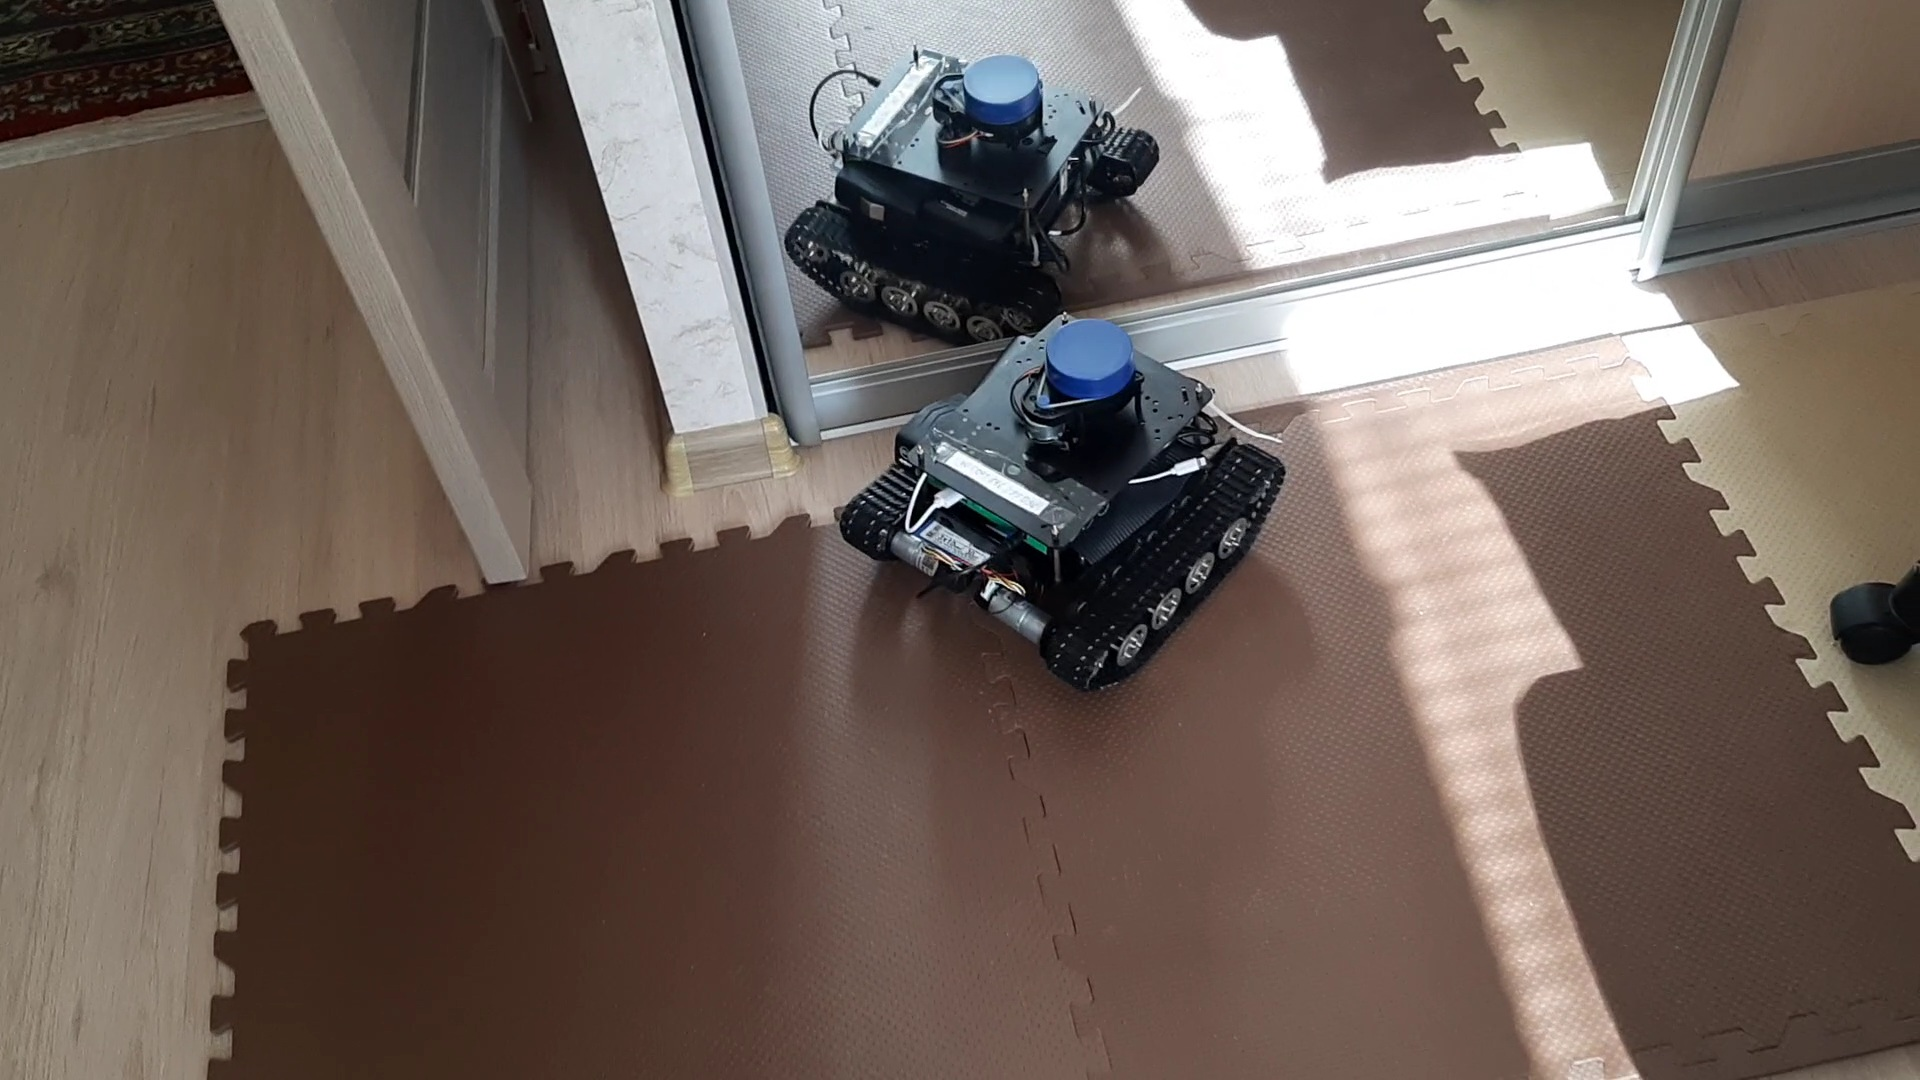
\includegraphics[width=1\linewidth]{robot-complete1.jpg} \\
  				\end{minipage}
  				\hfill
  				\begin{minipage}[b][][b]{0.32\linewidth}\centering
 					   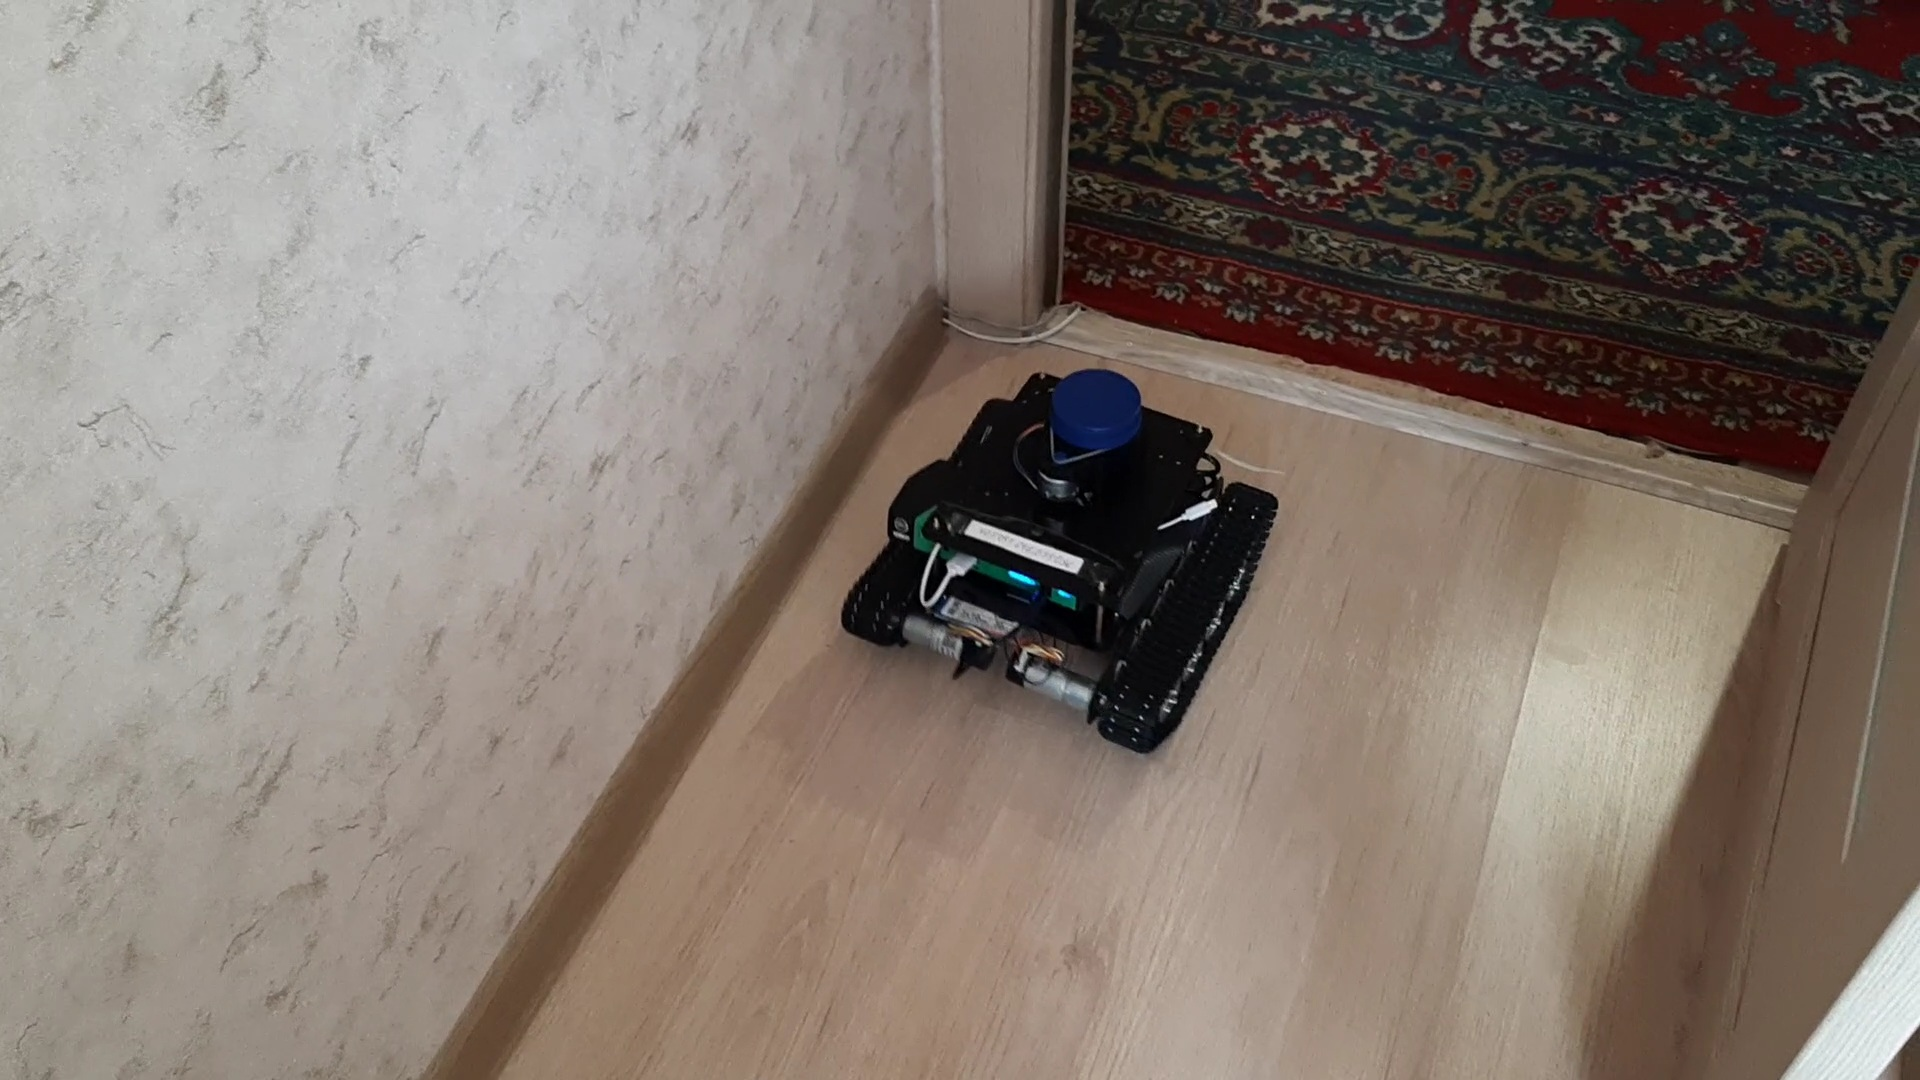
\includegraphics[width=1\linewidth]{robot-complete2.jpg} \\
 				 \end{minipage}
 				 \hfill
				  \begin{minipage}[b][][b]{0.32\linewidth}\centering
 					   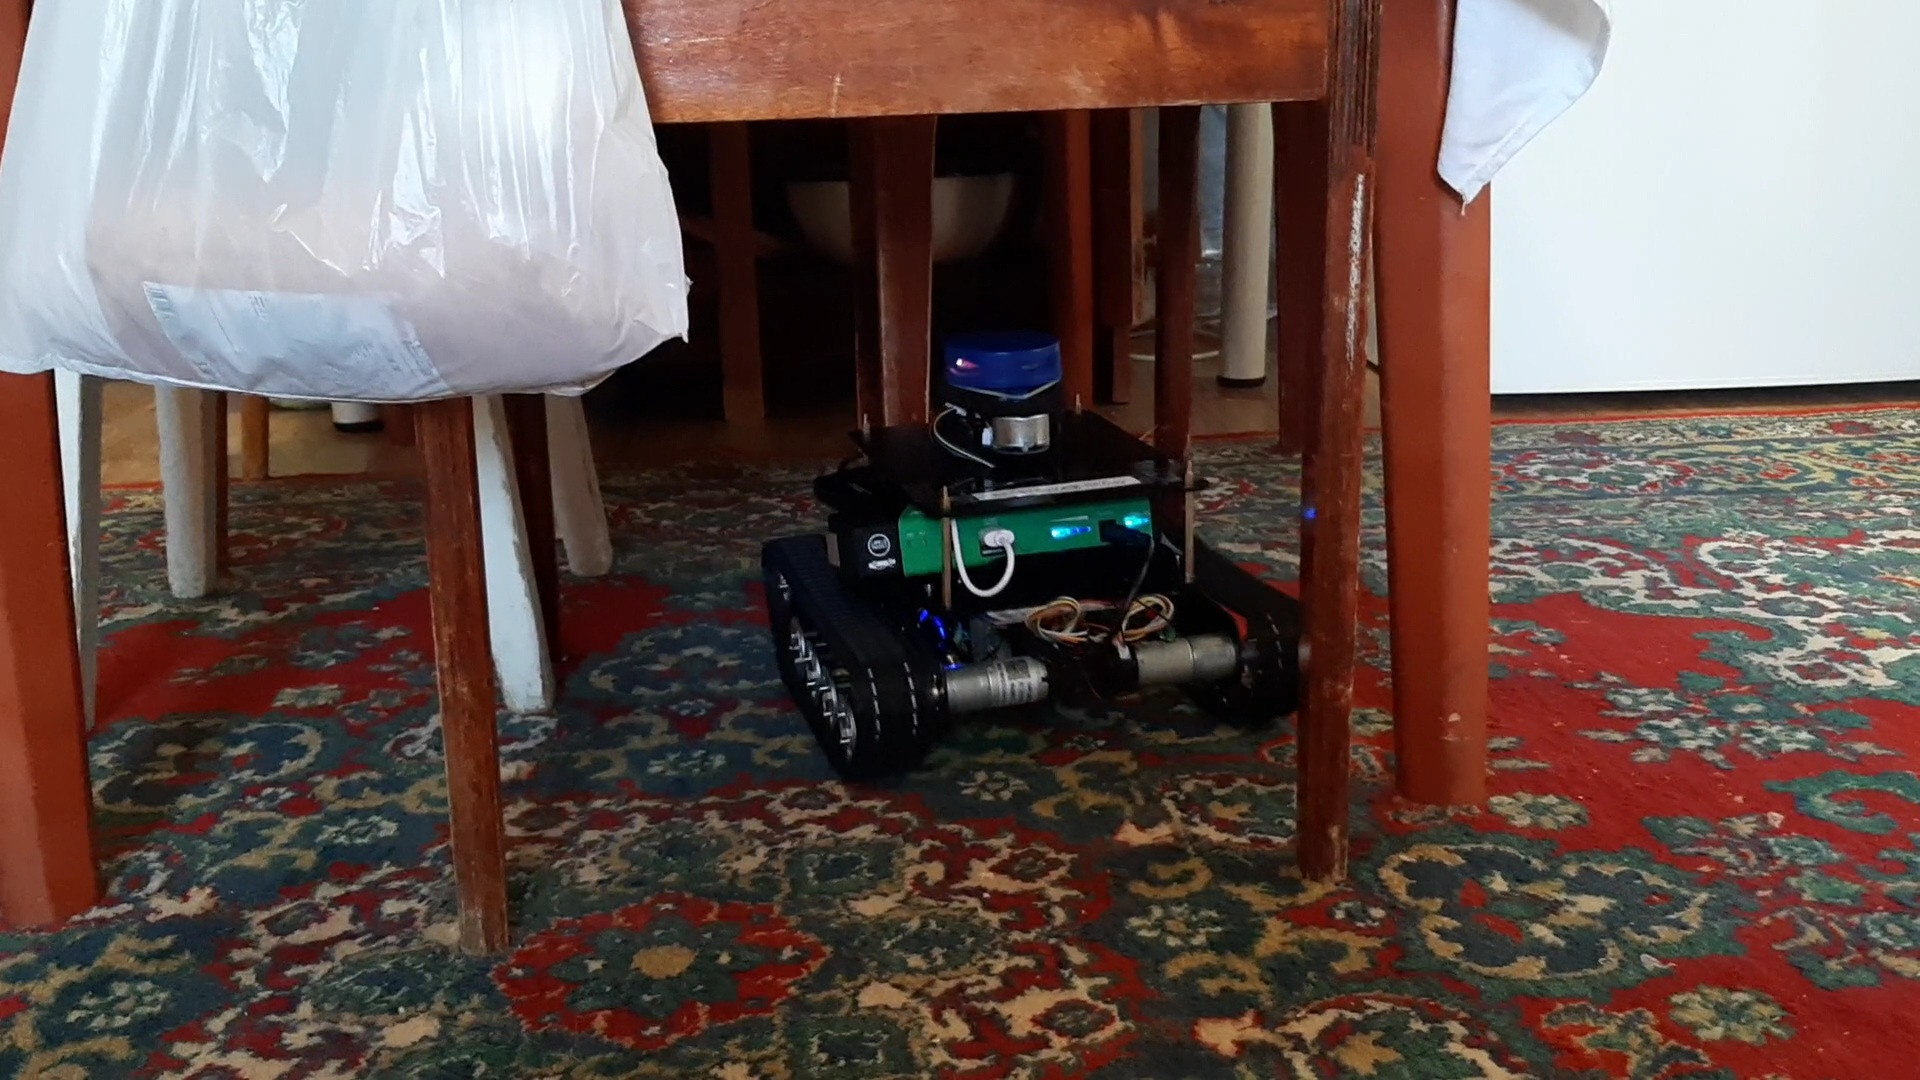
\includegraphics[width=1\linewidth]{robot-complete3.jpg} \\
  				 \end{minipage}
 				 \caption{Готовый робот, выполняющий поиск целевых объектов в доме.}
				  \label{fig:robot-complete}
			\end{figure}
			
			Разрабатываемому в рамках данной ВКР роботу посвящены такие англоязычные статьи как <<Recognition of Faces, Head Positions, Gender, Age, and Emotions In Real Time Using Deep Convolutional Neural Networks>> (представлена в рамках конференции YSIP3 2019 и уже имеется в базе данных Scopus) \cite{bib:YSIP-32019}, а также статья <<Autonomous Mobile Robot with AI based on Jetson Nano>> (будет представлена в рамках конференции FTC 2020 в этом году (статус accepted))\cite{bib:FTC2020}.
	
		\newpage

	\begin{thebibliography}{5}
		\bibitem{bib:AutomatizationRobotization} Сергеев, Е. Стратегия новой индустриализации России: автоматизация, роботизация, нанотехнологии. - ЛитРес, 2018. - 200 с. - Текст: непосредственный.
		\bibitem{bib:YSIP-32019} Kurbanov, E. Recognition of Faces, Head Positions, Gender, Age, and Emotions In Real Time Using Deep Convolutional Neural Networks. / CEUR-WS - URL: \url{http://ceur-ws.org/Vol-2500/#paper_4} (дата обращения: 28.12.2021). - Текст: электронный.
		\bibitem{bib:FTC2020} Kurbanov, E. Autonomous Mobile Robot with AI based on Jetson Nano. - Future Technologies Conference 2020. - Текст: непосредственный.
		\bibitem{bib:Thrun2004SimultaneousLA} Sebastian Thrun and Yufeng Liu and Daphne Koller and A. Ng and Zoubin Ghahramani and Hugh F. Durrant-Whyte. Simultaneous Localization and Mapping with Sparse Extended Information Filters. / The International Journal of Robotics Research, 2004. - c. 693 - 716, т. 23. - Текст: непосредственный.
		\bibitem{bib:TrajOptimizeLidarSLAM} Chen, Chunxu, Pei, Ling, Xu, Changqing, Danping, Zou, Qi, Yuhui, Zhu, Yifan, Li, Tao. Trajectory Optimization of LiDAR SLAM Based on Local Pose Graph. 10.1007/978-981-13-7751-8\_36, 2019 - Текст: непосредственный.
		\bibitem{bib:OdometrySLAM} S. A. S. Mohamed, M. Haghbayan, T. Westerlund, J. Heikkonen, H. Tenhunen, and J. Plosila, "A Survey on Odometry for Autonomous Navigation Systems," IEEE Access, vol. 7, pp. 97466-97486, 2019 - URL:\url{https://ieeexplore.ieee.org/stamp/stamp.jsp?arnumber=8764393} (дата обращения 30.12.2021). Текст: электронный.
		\bibitem{bib:ROSDescription} Quigley M. et al. ROS: an open-source Robot Operating System //ICRA workshop on open source software. – Т. 3. – №. 3.2. – С. 5, 2009 - URL: \url{http://robotics.stanford.edu/~ang/papers/icraoss09-ROS.pdf} (дата обращения 30.12.2021). Текст: электронный.
		\bibitem{bib:TS100Desc} szdoit Store, Описание товара <<Беспроводной металлический радиоуправляемый робот танк шасси амортизирующий автомобильный модуль с системой подвески гусеничная гусеница для Arduino игрушка «сделай сам» / AliExpress - URL: \url{https://aliexpress.ru/item/1005002054452153.html} (дата обращения 30.12.2021). - Текст: электронный.
		\bibitem{bib:TeensyDesc} PJRC, Teensy® 4.0 Development Board - URL: \url{https://www.pjrc.com/store/teensy40.html} (дата обращения 30.12.2021). Текст: электронный.
                \bibitem{bib:XavierNXDesc} Nvidia, Технические спецификации Nvidia Jetson Xavier NX. - URL: \url{https://www.nvidia.com/ru-ru/autonomous-machines/embedded-systems/jetson-xavier-nx/} (дата обращения: 30.12.2021). Текст: электронный.
                \bibitem{bib:YDLidarX4Desc} YDLIDAR, X4 DATA SHEET - URL: \url{https://www.ydlidar.com/Public/upload/files/2021-08-20/YDLIDAR%20X4%20Data%20sheet%20V2.0.pdf} (дата обращения 30.12.2021). Текст: электронный.
                \bibitem{bib:DT25-370Desc} Do Store, Описание товара DT25-370. - URL: \url{https://aliexpress.ru/item/4000548659629.html} (дата обращения: 30.12.2021). Текст: электронный.
	\end{thebibliography}
	
\end{document}